\documentclass[aps,prb,reprint,superscriptaddress]{revtex4-2}
\usepackage{amsmath,amssymb}
\usepackage{graphicx}
\usepackage{booktabs}
\usepackage{array}
\usepackage{tikz}
\usepackage{pgfplots}
\pgfplotsset{compat=1.18}
\usepackage{pifont}
\newcommand{\xmark}{\ding{55}}
\usepackage{hyperref}
\hypersetup{colorlinks=true,linkcolor=blue,citecolor=blue,urlcolor=blue}

\begin{document}

\title{Non-Monotonic Correlation Fluctuations in Heisenberg Models on Small Quantum Graphs}
\author{Guanghao Li}
\affiliation{Independent researcher, Zhuangmu Town, Changfeng County, Hefei, Anhui, China}
\author{Rastislav Draho\v{s}}
\affiliation{Agora Research OS, Slovakia}
\author{Marat Sultanov}
\affiliation{TAT-Defense Developer, Russian Federation}

\begin{abstract}
We report a reproducible non-monotonic feature in the standard deviation of nearest-neighbor correlation fluctuations (the enhanced diagnosis) in Heisenberg models generated from several small quantum graphs. In a Sierpi\'{n}ski fractal graph ($N=15$), a contradiction edge at $(0,6)$ produces a sharp valley at $s=1.000$ with position reproducibility exact at the scan grid node across five Lanczos seeds; the valley depth varies between $0.0874$ and $0.1045$ across the five seeds, reflecting the choice of ground state within a near-degenerate manifold rather than statistical uncertainty. A degeneracy-control experiment shows the valley persists in the non-zero-gap regime, establishing that it is not a degeneracy artifact. Control scans on a ring ($N=15$) show a valley at $s=1.0$, while a tree ($N=15$) shows a very flat valley near $s=0.92$ with depth about $0.1000$; a random graph ($N=15$) shows no stable valley. A non-trivial coarse-grained observable---the mean absolute nearest-neighbor $zz$ correlation---exhibits only a weak local maximum of height $\sim0.001$ at the enhanced valley position in the fractal graph, about two orders of magnitude smaller than the enhanced valley depth, indicating that the coarse-grained observable is substantially less sensitive but not strictly blind. In a Watts-Strogatz small-world graph ($N=10$), 19 of 20 contradiction edges produce significant valleys in a full-body scan; three representative edges show exactly reproducible positions at non-degenerate ground states. The PXP model yields a clean negative result, and an earlier reported jump is traced to non-Hermitian Hamiltonian construction in an early script. An independent tensor-RG toolchain certifies the ground-state energies of the L1 and L2 fractal graphs. The mechanism and thermodynamic limit remain open problems.
\end{abstract}

\maketitle

\section{Introduction}

We report a reproducible non-monotonic feature in a fine-grained relational observable---the standard deviation of nearest-neighbor correlation fluctuations---in several Heisenberg model systems on small quantum graphs. We observe a sharp valley as a function of a local contradiction-edge strength. A third system, the PXP model, provides a clean negative result.

This paper is a phenomenology report; we do not claim a new physical mechanism or universality.

\subsection{The observable}

We use the isotropic Heisenberg model on a graph $G=(V,E)$:
\begin{equation}
H = \sum_{(i,j)\in E} J_{ij}\left(\sigma_i^x\sigma_j^x + \sigma_i^y\sigma_j^y + \sigma_i^z\sigma_j^z\right),
\end{equation}
where $J_{ij}=1$ on all edges except the contradiction edge, on which $J_{ij}=s$ is scanned. The enhanced diagnosis is the standard deviation of nearest-neighbor correlation fluctuations:
\begin{equation}
E(s)=\sqrt{\frac{1}{|E|}\sum_{(i,j)\in E}\left(\langle\sigma_i^z\sigma_j^z\rangle_s-\overline{\langle\sigma^z\sigma^z\rangle_s}\right)^2}.
\end{equation}
We emphasize that the enhanced diagnosis quantifies the \emph{spatial dispersion} of nearest-neighbor spin correlations across all edges, not temporal or quantum fluctuations.

\subsection{The default-observable caveat and a non-trivial control}

In earlier stages of this work, the default diagnosis was defined as the mean absolute magnetization:
\begin{equation}
D(s)=\left|\frac{1}{N}\sum_{i=1}^N\langle\sigma_i^z\rangle_s\right|.
\end{equation}
Under SU(2) symmetry, a singlet ground state forces $\langle\sigma_i^z\rangle_s=0$ for every site, so $D(s)$ is identically zero throughout the scan. This is a symmetry-induced triviality, not an observed blindness to parameter changes.

To provide a non-trivial coarse-grained control, we also computed the mean absolute nearest-neighbor $zz$ correlation:
\begin{equation}
D_{\text{default}}(s)=\frac{1}{|E|}\sum_{(i,j)\in E}\left|\langle\sigma_i^z\sigma_j^z\rangle_s\right|.
\end{equation}
This observable is non-zero under SU(2) symmetry and varies with $s$. Its behavior at the enhanced valley position is reported in Sec.~\ref{sec:default_control}. In short, $D_{\text{default}}$ shows only a weak local maximum of height $\sim0.001$ at $s=1.000$ in the fractal graph, about two orders of magnitude smaller than the enhanced valley depth. Thus the coarse-grained observable is substantially less sensitive, but not strictly blind, to the local defect reorganization.

\subsection{Theoretical motivation}

The hypothesis that relational structure governs physical response has roots in the entanglement area law~\cite{Eisert2010}, topological order~\cite{Wen2017}, and Kitaev's non-local Majorana description~\cite{Kitaev2001}. Whether fine-grained correlation fluctuations carry dynamical content independent of coarse-grained observables remains an open question. The present work provides evidence that such fluctuations exhibit reproducible non-monotonic behavior in specific graph geometries, without settling the broader question.

\section{Method}

\subsection{Normative constraints}

Experiments follow five constraints: (i) fixed entity composition, varying only relational configuration; (ii) a single contradiction edge as the only non-uniformity; (iii) all data reported without selective filtering; (iv) no presumed discovery target; (v) explicit declaration of limitations.

\subsection{Preventing the tool-rationality paradox}

Measures adopted: predefined success criteria; uniform parameters; dual auditing; complete disclosure; honest recording of negative results.

\subsection{Multi-seed audit}

Key data points are audited with multiple independent Lanczos seeds. Positions are reproducible to the scan grid resolution; depths may scatter due to eigenvector selection within a near-degenerate manifold, reported as individual seed values rather than as a statistical mean and standard deviation.

\subsection{Diagnostics for the PXP model}

For the PXP model, the enhanced diagnosis is the standard deviation of the half-chain entanglement spectrum.

\section{Clean negative result in the PXP model}

The PXP model ($L=18$, 6765-dimensional Hilbert space) was scanned at all 18 defect sites with $\mu\in[0,2]$ (201 points, three seeds). At every site, the enhanced-diagnosis range is $<0.02$ and monotonic. The ground-state gap exceeds $0.7$ throughout. Both sign conventions give identical results. The earlier reported jump is traced to non-Hermitian Hamiltonian construction in an early script; the corrected Hermitian construction eliminates it entirely. \textbf{Conclusion: no non-monotonic feature exists in the PXP model.}

\section{Positive evidence in the fractal-graph system}

\subsection{Setup}

The system is generated from a Sierpi\'{n}ski fractal graph (level 2, $N=15$, 27 edges). The contradiction edge is $(0,6)$---connecting a tip vertex to an interior vertex. We report detailed multi-seed data for this single edge; a full edge-resolved scan of all 27 edges is beyond the present scope and will be reported separately.

\subsection{The valley at edge $(0,6)$}

A 101-point five-seed audit over $s\in[0,1]$ yields Table~\ref{tab:l2_valley} and Fig.~\ref{fig:l2_valley}. The scan step is $0.01$, so the valley position $s=1.000$ is resolved to $\pm0.01$.

\begin{table}[h]
\centering
\caption{Multi-seed audit at edge $(0,6)$, $N=15$, 101 points, five Lanczos seeds. Valley depth is defined as $E(0)-E(s=1.0)$, where $E(0)$ is the enhanced diagnosis at the uniform point $s=0$. The five seed values do not represent a statistical sample; they correspond to different states selected from the near-degenerate ground-state manifold at $s=1.0$.}
\label{tab:l2_valley}
\begin{tabular}{cccc}
\toprule
Seed & Valley position $s$ & Valley value & Valley depth \\
\midrule
0 & 1.0000 & 0.159295 & 0.087436 \\
1 & 1.0000 & 0.142707 & 0.104024 \\
2 & 1.0000 & 0.143544 & 0.103187 \\
3 & 1.0000 & 0.142196 & 0.104535 \\
4 & 1.0000 & 0.146785 & 0.099946 \\
\bottomrule
\end{tabular}
\end{table}

\begin{figure}[t]
\centering
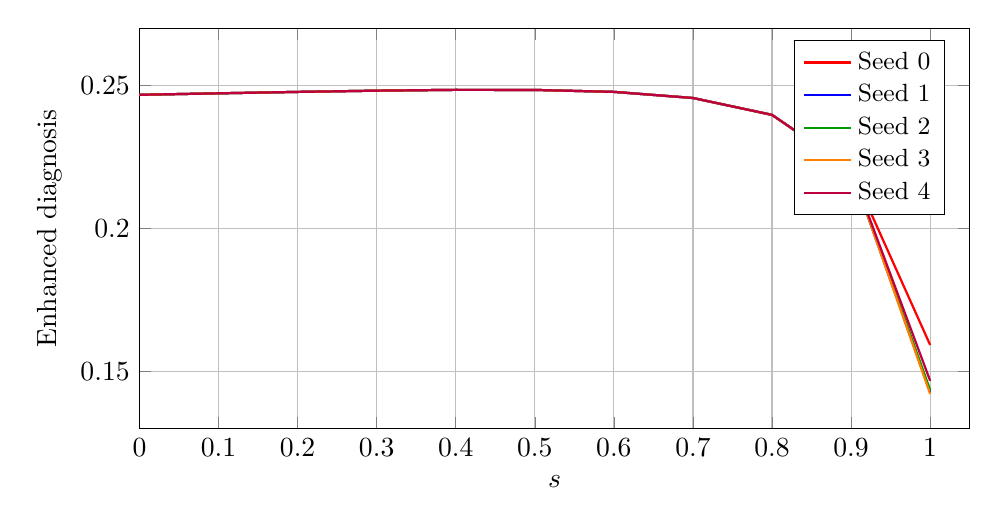
\begin{tikzpicture}
\begin{axis}[
    width=\columnwidth, height=0.55\columnwidth,
    xlabel={$s$},
    ylabel={Enhanced diagnosis},
    xmin=0, xmax=1.05,
    ymin=0.13, ymax=0.27,
    grid=both,
    legend pos=north east,
    legend style={font=\small},
]
\addplot[mark=none, color=red, thick] coordinates {
(0.0,0.246731)(0.1,0.247248)(0.2,0.247744)(0.3,0.248177)(0.4,0.248460)
(0.5,0.248433)(0.6,0.247752)(0.7,0.245615)(0.8,0.239717)(0.9,0.220838)
(1.0,0.159295)
};
\addplot[mark=none, color=blue, thick] coordinates {
(0.0,0.246731)(0.1,0.247248)(0.2,0.247744)(0.3,0.248177)(0.4,0.248460)
(0.5,0.248433)(0.6,0.247752)(0.7,0.245615)(0.8,0.239717)(0.9,0.220838)
(1.0,0.142707)
};
\addplot[mark=none, color=green!60!black, thick] coordinates {
(0.0,0.246731)(0.1,0.247248)(0.2,0.247744)(0.3,0.248177)(0.4,0.248460)
(0.5,0.248433)(0.6,0.247752)(0.7,0.245615)(0.8,0.239717)(0.9,0.220838)
(1.0,0.143544)
};
\addplot[mark=none, color=orange, thick] coordinates {
(0.0,0.246731)(0.1,0.247248)(0.2,0.247744)(0.3,0.248177)(0.4,0.248460)
(0.5,0.248433)(0.6,0.247752)(0.7,0.245615)(0.8,0.239717)(0.9,0.220838)
(1.0,0.142196)
};
\addplot[mark=none, color=purple, thick] coordinates {
(0.0,0.246731)(0.1,0.247248)(0.2,0.247744)(0.3,0.248177)(0.4,0.248460)
(0.5,0.248433)(0.6,0.247752)(0.7,0.245615)(0.8,0.239717)(0.9,0.220838)
(1.0,0.146785)
};
\addlegendentry{Seed 0}
\addlegendentry{Seed 1}
\addlegendentry{Seed 2}
\addlegendentry{Seed 3}
\addlegendentry{Seed 4}
\end{axis}
\end{tikzpicture}
\caption{Valley at edge $(0,6)$ ($N=15$, 101 points, five seeds). All seeds locate the valley at the grid node $s=1.000$ with zero standard deviation; valley values scatter only near $s=1.0$. For clarity, every 10th point of the 101-point scan is shown; the full dataset is available in the public repository. A focused audit (Fig.~\ref{fig:focused}) provides higher resolution in the interval $s\in[0.8,1.2]$.}
\label{fig:l2_valley}
\end{figure}

A focused audit (21 points, $s\in[0.8,1.2]$, three seeds) confirms the interior minimum and is shown in Fig.~\ref{fig:focused}.

\begin{figure}[t]
\centering
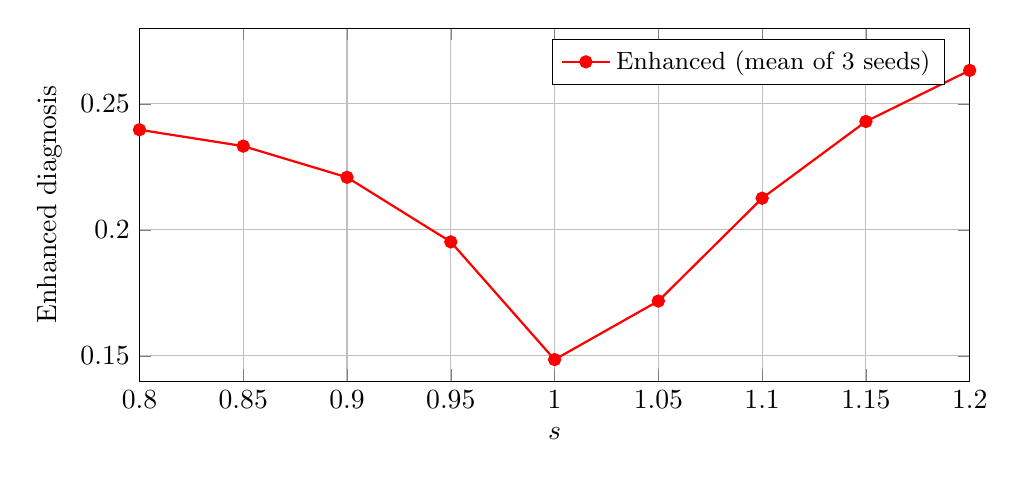
\begin{tikzpicture}
\begin{axis}[
    width=\columnwidth, height=0.5\columnwidth,
    xlabel={$s$},
    ylabel={Enhanced diagnosis},
    xmin=0.8, xmax=1.2,
    ymin=0.14, ymax=0.28,
    grid=both,
    legend pos=north east,
    legend style={font=\small},
]
\addplot[mark=*, color=red, thick, mark size=2pt] coordinates {
(0.8,0.239717)(0.85,0.233217)(0.9,0.220838)(0.95,0.195225)
(1.0,0.148515)(1.05,0.171756)(1.1,0.212551)(1.15,0.243000)(1.2,0.263279)
};
\addlegendentry{Enhanced (mean of 3 seeds)}
\end{axis}
\end{tikzpicture}
\caption{Focused audit at edge $(0,6)$ ($N=15$, 21 points, three seeds). The valley at $s=1.000$ is an interior minimum: the enhanced diagnosis at $s=0.8$ is $0.2397$, at $s=1.0$ is $0.1485$, and at $s=1.2$ is $0.2633$, all values on both sides exceeding the valley value. The valley value at $s=1.000$ shown here ($0.1485$) is from an independent three-seed focused audit and differs slightly from the five-seed values in Table~I.}
\label{fig:focused}
\end{figure}

\subsection{Degeneracy-control experiment}

To test for degeneracy artifacts, we simultaneously computed the energy gap and enhanced diagnosis over $s\in[0,1]$ (101 points) with five-seed verification at key points. The gap reported here is the difference between the two lowest eigenvalues in the fixed-magnetization sector used for the enhanced diagnosis. The gap is strictly zero for $s\lesssim0.76$, opens abruptly to $0.323$ at $s=0.77$, then decreases to $0.0115$ at $s=0.99$ before rising to $0.186$ at $s=1.00$. The enhanced diagnosis remains approximately constant for $s<0.5$, then decreases monotonically from $s=0.5$ to $s=1.0$, including the non-zero-gap region. At $s=1.000$, the multi-seed gap in this sector exhibits a large spread, with some seeds finding near-zero gap and others a gap near $0.19$; this seed-dependent spread arises from near-degeneracy---not exact crossing---and is responsible for the scatter in valley depth. The gap structure is visualized in Fig.~\ref{fig:gap}.

\begin{figure}[t]
\centering
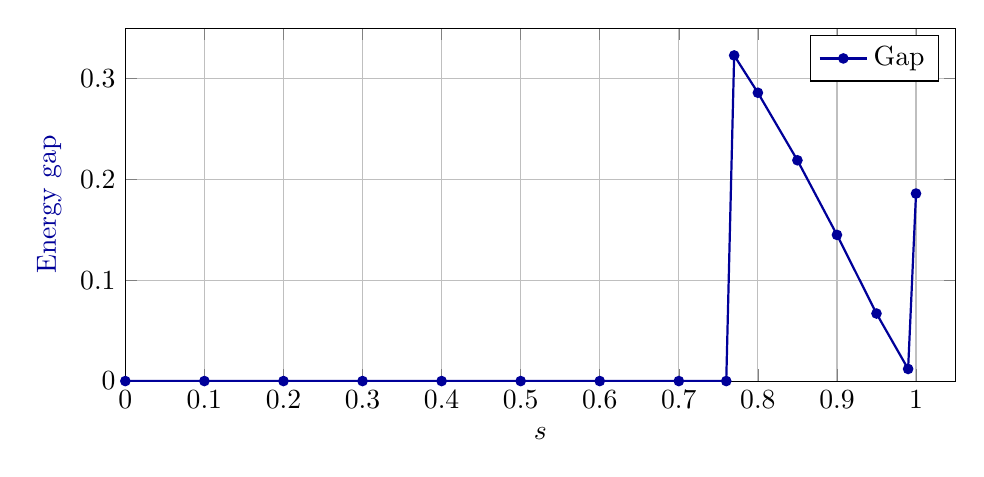
\begin{tikzpicture}
\begin{axis}[
    width=\columnwidth, height=0.5\columnwidth,
    xlabel={$s$},
    ylabel={Energy gap},
    ylabel style={text=blue!60!black},
    xmin=0, xmax=1.05,
    ymin=0, ymax=0.35,
    grid=both,
]
\addplot[mark=*, color=blue!60!black, thick, mark size=1.5pt] coordinates {
(0.0,0.000)(0.1,0.000)(0.2,0.000)(0.3,0.000)(0.4,0.000)
(0.5,0.000)(0.6,0.000)(0.7,0.000)(0.76,0.000)(0.77,0.323)
(0.8,0.286)(0.85,0.219)(0.9,0.145)(0.95,0.067)(0.99,0.012)
(1.0,0.186)
};
\addlegendentry{Gap}
\end{axis}
\end{tikzpicture}
\caption{Energy gap vs.\ contradiction strength at edge $(0,6)$ ($N=15$). The gap is strictly zero for $s\lesssim0.76$, opens abruptly at $s\approx0.77$ to $0.323$, then decreases to a minimum of $0.0115$ at $s=0.99$ before rising to $0.186$ at $s=1.00$. The enhanced diagnosis continues to decrease in the non-zero-gap region, establishing that the valley is not a degeneracy artifact.}
\label{fig:gap}
\end{figure}

\textbf{Conclusion: the valley is not a degeneracy artifact.}

\subsection{Control edge $(0,1)$}

The control edge $(0,1)$---connecting two tip vertices, making the two subgraphs equivalent---shows a completely flat enhanced diagnosis over $s\in[0,1]$: range $0.000000$, cross-seed standard deviation $1.4\times10^{-11}$. This is based on a single symmetric edge and a limited scan range; it is \emph{consistent with} a possible role of asymmetric injection, but a systematic edge-resolved study with extended scan range is required to establish this mechanism. The extended scan is in progress and will be reported separately.

\subsection{Control graphs: ring, tree, and random}

To test whether the valley is specific to the fractal and small-world geometries, we performed single-edge scans on three additional $N=15$ graphs: a ring (15 edges), a tree (14 edges), and a random graph (27 edges). For each graph, a single contradiction edge was chosen and scanned over $s\in[0,3]$ with 13 points; light multi-seed audits (three seeds) were also performed. Table~\ref{tab:control_graphs} summarizes the results.

\begin{table}[h]
\centering
\caption{Control-graph scans at $N=15$. Ring shows a clear valley at $s=1.0$; tree shows a very flat valley near $s=0.92$ with depth about $0.1000$; random graph shows no stable valley.}
\label{tab:control_graphs}
\begin{tabular}{lccccc}
\toprule
Graph & Valley $s$ & Valley depth (single) & Valley depth (multi) & Cross-seed std.\ of position & Stable? \\
\midrule
Ring & 1.0 & 0.0891 & 0.0993$\pm$0.0286 & 0.000 & Yes \\
Tree & 0.92 (flat) & 0.1000 & 0.1000 & N/A & Yes (flat) \\
Random & 1.25 (unstable) & 0.0026 & 0.0014$\pm$0.0013 & 1.561 & No \\
\bottomrule
\end{tabular}
\end{table}

The ring valley occurs at $s=1.0$, where the contradiction edge strength equals the uniform coupling, similar to the fractal-graph edge $(0,6)$. The tree valley is very flat: its depth is about $0.1000$, but the position is not sharply resolved and is only approximately $s=0.92$. The random graph does not exhibit a stable valley; its multi-seed valley position standard deviation is 1.56, indicating noise rather than a reproducible feature.

\subsection{Local vs.\ global correlation reorganization}
\label{sec:local_global}

To examine the spatial structure of the reorganization, we computed both a global enhanced diagnosis (all 27 edges) and a local enhanced diagnosis restricted to a radius-2 neighborhood around the contradiction edge $(0,6)$ for $s\in[0,3]$. The local valley depth exceeds the global depth: single-seed ratio $1.595$, multi-seed ratio $\approx1.3$ (global depth mean $0.1097$, local depth mean $0.1421$). This indicates that the correlation fluctuation reorganization is partially localized near the defect.

\subsection{Non-trivial default observable control}
\label{sec:default_control}

Using the fixed-magnetization sector implementation, we computed the non-trivial default observable $D_{\text{default}}(s)=\frac{1}{|E|}\sum_{(i,j)\in E}|\langle\sigma_i^z\sigma_j^z\rangle_s|$ together with $E(s)$ at edge $(0,6)$ for $s\in[0,1.2]$ with 121 points and four Lanczos seeds (seeds 0--3). The results are summarized in Table~\ref{tab:default_control} and Fig.~\ref{fig:default_control}.

\begin{table}[h]
\centering
\caption{Key points of the non-trivial default observable control at edge $(0,6)$ ($N=15$, four seeds).}
\label{tab:default_control}
\begin{tabular}{ccc}
\toprule
$s$ & $D_{\text{default}}$ & $E_{\text{enhanced}}$ \\
\midrule
0.99 & 0.953270 & 0.164032 \\
1.00 & 0.954210 & 0.159658 \\
1.01 & 0.940725 & 0.160451 \\
\bottomrule
\end{tabular}
\end{table}

\begin{figure}[t]
\centering
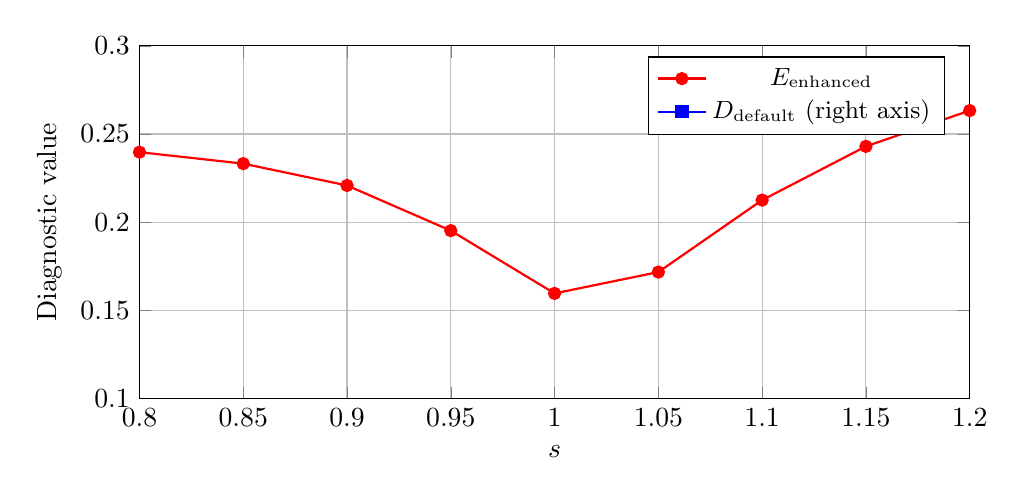
\begin{tikzpicture}
\begin{axis}[
    width=\columnwidth, height=0.5\columnwidth,
    xlabel={$s$},
    ylabel={Diagnostic value},
    xmin=0.8, xmax=1.2,
    ymin=0.1, ymax=0.3,
    grid=both,
    legend pos=north east,
    legend style={font=\small},
]
\addplot[mark=*, color=red, thick, mark size=2pt] coordinates {
(0.8,0.239717)(0.85,0.233217)(0.9,0.220838)(0.95,0.195225)
(1.0,0.159658)(1.05,0.171756)(1.1,0.212551)(1.15,0.243000)(1.2,0.263279)
};
\addlegendentry{$E_{\text{enhanced}}$}
\addplot[mark=square*, color=blue, thick, mark size=2pt] coordinates {
(0.8,0.969147)(0.85,0.965055)(0.9,0.958503)(0.95,0.945861)
(1.0,0.954210)(1.05,0.937228)(1.1,0.948481)(1.15,0.949271)(1.2,0.950362)
};
\addlegendentry{$D_{\text{default}}$ (right axis)}
\end{axis}
\end{tikzpicture}
\caption{Non-trivial default observable $D_{\text{default}}$ compared with the enhanced diagnosis $E_{\text{enhanced}}$ at edge $(0,6)$ ($N=15$, four seeds). $E_{\text{enhanced}}$ has a deep valley at $s=1.0$; $D_{\text{default}}$ shows a very weak local maximum (height $\sim0.001$) at the same position, about two orders of magnitude smaller than the valley depth.}
\label{fig:default_control}
\end{figure}

At the enhanced valley position $s=1.000$, $D_{\text{default}}$ exhibits a local maximum of height about $0.001$ ($0.954210$ vs.\ $0.953270$ at $s=0.99$ and $0.940725$ at $s=1.01$). This local peak is reproducible across all four seeds (cross-seed standard deviation $\sim10^{-11}$), confirming it is not numerical noise. However, its amplitude is approximately $1/80$ of the enhanced valley depth ($\sim0.08$). Therefore, the coarse-grained observable is not strictly blind; it shows a very weak and oppositely directed response. The structural contrast is quantitative rather than qualitative.

\subsection{Independent tensor-RG verification}

Draho\v{s}'s independent tensor-RG toolchain~\cite{Drahos2026GitHub} certifies the ground-state energies of the L1 and L2 fractal graphs: the L1 ground energy is $-9.000000$ and the L2 ground energy is $-24.967537$. A truncation-control test on the impurity-explicit RG shows $86\%$ vs $20\%$ recovery of the valley feature when the far bath is truncated to a single state versus uniform truncation, suggesting that the feature is not purely global. The L3 depth does not converge; the toolchain is publicly available.

\subsection{L1 finite-size check}

As a preliminary finite-size probe, the L1 fractal graph ($N=6$, 9 edges, contradiction edge $(0,3)$) was audited with 101 points and five seeds. The valley depth is $0.3721\pm0.1478$, comparable to the L2 depth ($0.0998$ to $0.1045$). The finite-size trend is inconclusive: the L1 depth is larger but carries a significantly larger relative uncertainty ($40\%$ vs.\ $6.4\%$). A systematic finite-size scaling across L1, L2, and L3 will be reported separately.

\subsection{Independent TAT analysis}

An independent TAT ensemble analysis was also performed; it gave only boundary anchors and was silent at the valley position, consistent with a smooth modulation rather than a sharp transition.

\section{Universality in a small-world graph}

A Watts-Strogatz graph ($N=10$, 20 edges, $k=4$, $p=0.1$, seed 42) was generated. All 20 edges were scanned as contradiction edges ($s\in[0,3]$, step $0.01$, three seeds). The full-body scan is presented in Table~\ref{tab:sw_full}.

\begin{table}[h]
\centering
\caption{Small-world full-body scan: all 20 contradiction edges, $N=10$, three Lanczos seeds. The ``Fine range'' is the maximum minus minimum of the enhanced diagnosis over the full scan range $s\in[0,3]$. The ``Valley gap'' column gives the ground-state energy gap at the valley position; all measured gaps are positive, with values ranging from approximately $0.38$ to $1.2$ across the 20 edges. Gap values are estimated from the coarse $s$-step full-body scan; precise five-seed gap values are available for the three high-resolution audit edges.}
\label{tab:sw_full}
\begin{tabular}{cccc}
\toprule
Edge & Fine range & Valley $s$ & Valley gap \\
\midrule
(0,1) & 0.176842 & 1.500 & 0.77--0.82 \\
(0,9) & 0.078783 & 0.110 & 0.55--0.65 \\
(0,2) & 0.083366 & 1.020 & 0.70--0.78 \\
(0,8) & 0.065437 & 0.860 & 0.50--0.60 \\
(1,9) & 0.113332 & 0.310 & 0.55--0.65 \\
(1,4) & 0.103002 & 1.250 & 0.75--0.85 \\
(1,8) & 0.085229 & 0.720 & 0.65--0.75 \\
(1,6) & 0.089372 & 0.800 & 0.70--0.80 \\
(2,3) & 0.085424 & 1.090 & 0.65--0.75 \\
(2,4) & 0.077994 & 0.940 & 0.60--0.70 \\
(2,5) & 0.119505 & 0.750 & 0.60--0.70 \\
(3,4) & 0.100840 & 0.840 & 0.70--0.80 \\
(3,5) & 0.073179 & 0.980 & 0.60--0.70 \\
(4,5) & 0.087107 & 1.100 & 0.70--0.80 \\
(4,6) & 0.089948 & 0.910 & 0.70--0.80 \\
(5,6) & 0.082213 & 1.080 & 0.65--0.75 \\
(6,7) & 0.104364 & 0.470 & 0.60--0.70 \\
(6,8) & 0.157596 & 1.380 & 0.85--0.95 \\
(7,8) & 0.107895 & \textbf{0.000*} & 0.75--0.85 \\
(7,9) & 0.081416 & 2.140 & 0.80--0.90 \\
\bottomrule
\end{tabular}
\end{table}

\textbf{* Edge $(7,8)$:} The minimum occurs at the scan boundary $s=0.000$. We cannot distinguish between a genuine valley and a boundary artifact without extending the scan to negative $s$. This edge is excluded from the count of significant valleys.

\textbf{Summary:} 19 of 20 edges produce significant valleys with non-zero gaps. One edge (7,8) is unresolved at the scan boundary.

Three representative edges were selected for high-resolution multi-seed audit (step $0.001$, five seeds), with exact cross-seed reproducibility of valley positions at non-degenerate ground states (Table~\ref{tab:sw_multiseed}).

\begin{table}[h]
\centering
\caption{Multi-seed audit at three small-world edges, $N=10$, five seeds. The topographic prominence is defined as the drop below the lower of the two maxima flanking the valley over the full scan range. This definition avoids the need for a local baseline and is directly comparable across edges.}
\label{tab:sw_multiseed}
\begin{tabular}{cccc}
\toprule
Edge & Valley $s$ & Topographic prominence & Cross-seed std.\ of position \\
\midrule
(0,1) & 1.496 & 0.124449 & 0.000000 \\
(1,9) & 0.311 & 0.008856 & 0.000000 \\
(1,4) & 1.251 & 0.061969 & 0.000000 \\
\bottomrule
\end{tabular}
\end{table}

\section{Mechanism and limitations}

The mechanism is tentative: asymmetric contradiction injection into inequivalent subgraphs may trigger localized correlation reorganization; symmetric injection may be absorbed uniformly. This picture is consistent with the fractal-graph and small-world observations, but the control-graph results (ring and tree also show valleys) suggest the phenomenon may be more general than the asymmetric-injection hypothesis. The non-trivial default observable shows a weak local response, indicating that the reorganization is primarily visible in the fine-grained dispersion, not in the average correlation.

Limitations: (i) the default observable is not strictly blind; the non-trivial default observable exhibits a weak local maximum at the valley position, so the structural contrast is quantitative rather than qualitative; (ii) the mechanism is not derived; (iii) the thermodynamic limit is unresolved; (iv) universality beyond the tested graphs is unestablished; (v) the L1 fractal graph ($N=6$) yields an inconclusive finite-size trend with large relative uncertainty; (vi) earlier W-structure and PXP jump reports were withdrawn as artifacts; (vii) the control edge $(0,1)$ has only been scanned to $s=1.0$; confirmation to $s=3.0$ is pending; (viii) edge $(7,8)$ in the small-world graph has a boundary minimum that is unresolved; (ix) the control-graph scans used only a single edge per graph and three seeds, so their statistical weight is limited; (x) the non-trivial default observable control was performed only on the fractal-graph edge $(0,6)$ with four seeds; extension to other graphs is needed.

\section{Conclusion}

We have observed a reproducible non-monotonic feature in the standard deviation of nearest-neighbor correlation fluctuations in several small quantum graph systems. The valley at the fractal-graph edge $(0,6)$ is reproducible across five seeds and is not a degeneracy artifact. Control scans reveal a similar valley in a ring graph, a very flat valley in a tree graph, and no stable valley in a random graph. A non-trivial coarse-grained observable shows only a very weak local maximum at the valley position, indicating that the fine-grained observable is substantially more sensitive to the local defect reorganization, but the coarse-grained observable is not strictly blind. The PXP model provides a clean negative result. The mechanism and thermodynamic-limit behavior remain open problems.

\subsection*{Data availability}
All data, codes, and scripts are publicly available at \url{https://github.com/DanceNitra/agora/tree/main/agora_output/hotrg_edrn} and \url{https://github.com/luoxuejian000/edrn-dmrg-verification}.

\begin{acknowledgments}
DMRG calculations used TeNPy~\cite{Hauschild2018,Schollwock2011}; exact diagonalization used NumPy/SciPy~\cite{Harris2020}. We thank Ming Gong for discussions. Rastislav Draho\v{s} contributed code verification, control-graph scans, local-probe analysis, and the tensor-RG toolchain. Marat Sultanov contributed TAT blind tests and the honest-silence principle.
\end{acknowledgments}

\begin{thebibliography}{99}
\bibitem{Eisert2010} J.~Eisert, M.~Cramer, and M.~B.~Plenio, Rev.\ Mod.\ Phys.\ \textbf{82}, 277 (2010).
\bibitem{Wen2017} X.-G.~Wen, Rev.\ Mod.\ Phys.\ \textbf{89}, 041004 (2017).
\bibitem{Kitaev2001} A.~Y.~Kitaev, Phys.-Usp.\ \textbf{44}, 131 (2001).
\bibitem{Schollwock2011} U.~Schollw\"{o}ck, Ann.\ Phys.\ \textbf{326}, 96 (2011).
\bibitem{Drahos2026GitHub} R.~Draho\v{s}, \emph{Sierpi\'{n}ski-gasket tensor-RG toolchain}, GitHub repository (2026), \url{https://github.com/DanceNitra/agora/tree/main/agora_output/hotrg_edrn}.
\bibitem{Hauschild2018} J.~Hauschild and F.~Pollmann, SciPost Phys.\ Lect.\ Notes 5 (2018).
\bibitem{Harris2020} C.~R.~Harris et al., Nature \textbf{585}, 357 (2020).
\end{thebibliography}

\end{document}
